\documentclass[12pt,a4paper]{article}
\usepackage[utf8]{inputenc}
%Set page layout parameters
\usepackage[
top=4cm,
bottom=2cm,
left=2cm,
right=2cm,
headheight=2cm,
footskip=1cm,
marginparwidth=2cm]{geometry}
\usepackage[dvipsnames]{xcolor}
% To use color boxes
\usepackage{tcolorbox}
\usepackage{lipsum}
\tcbuselibrary{listings,theorems,skins,vignette,raster,breakable,magazine,poster,fitting,hooks}
\newcounter{ejemplo}
%Images path
\graphicspath{{images/}}
\usepackage{float} %provide us with the option H
\usepackage{fancyhdr}
\usepackage{tikz}
\usepackage{tikzpagenodes}
%to redefine figure caption 
\renewcommand{\figurename}{Figura}
%change text font
\usepackage[T1]{fontenc}
\usepackage{tgbonum} % LaTeX will use the TEX Gyre Bonum font family
\usepackage{amssymb}


\definecolor{subtitle_yellow}{RGB}{252,213,129}
\definecolor{title_yellow}{RGB}{249,175,16}
\definecolor{steel_blue_title}{RGB}{93,138,168}
\definecolor{pewter_blue_subtitle}{RGB}{149,178,198}
\definecolor{ecru_circle}{RGB}{215,190,130}
\definecolor{ecru_circle1}{RGB}{68,148,173}

\newcommand{\myfirststyle}{%
	\begin{tikzpicture}[remember picture, overlay]
		
		%top border
		\fill[fill=steel_blue_title](current page.north west) rectangle ([yshift=-15mm]current page.north east);
		
		\fill[fill=pewter_blue_subtitle]([yshift=-17mm]current page.north west) rectangle ([yshift=-30mm]current page.north east);
		
		%page box
		%\draw[lightgray, fill=Rhodamine, fill opacity=0.05, line width=1mm, rounded corners=3mm] ([xshift=-5mm,yshift=5mm]current page text area.north west) rectangle ([xshift=5mm,yshift=-5mm]current page text area.south east);
		
		%bottom box
		\fill[fill=pewter_blue_subtitle](current page.south west) rectangle ([yshift=10mm]current page.south east);
		
		%page circle
		\draw[white,fill=ecru_circle1,line width=2mm] ([xshift=-5mm,yshift=25mm]current page text area.north east) circle (1); 
		
		
		%page number text        
		%\node[anchor=center] at ([xshift=-5mm,yshift=25mm]current page text area.north east) {\Huge\bfseries\sffamily\color{white}{\thepage}};
		
		%title text
		\node[anchor=west] at ([yshift=32mm]current page text area.north west) {\Huge\bfseries\sffamily\color{white}{Multiplicador de capacitancia}};
		
		%subtitle text
		\node[anchor=west] at ([xshift=10mm,yshift=16mm]current page text area.north west) {\Large\bfseries\sffamily\color{white}{}};
		
		%footer text
		\node[anchor=center] at ([yshift=-15mm]current page text area.south) {\large\bfseries\sffamily\color{white}{Created by: Rodrigo Castillejos}};
		
	\end{tikzpicture}
}


%create page style
\fancypagestyle{MyFirstStyle}{%
	\fancyhf{}
	\fancyhead[C]{\myfirststyle}
	\renewcommand{\headrulewidth}{0pt}
}%

\pagestyle{MyFirstStyle}

\colorlet{colexam}{red!75!black}
\newtcolorbox[use counter=ejemplo]{myexample}{%
	empty,title={Ejemplo \thetcbcounter},attach boxed title to top left,
	boxed title style={empty,size=minimal,toprule=2pt,top=4pt,
		overlay={\draw[colexam,line width=2pt]
			([yshift=-1pt]frame.north west)--([yshift=-1pt]frame.north east);}},
	coltitle=colexam,fonttitle=\Large\bfseries,
	before=\par\medskip\noindent,parbox=false,boxsep=0pt,left=0pt,right=3mm,top=4pt,
	breakable,pad at break*=0mm,vfill before first,
	overlay unbroken={\draw[colexam,line width=1pt]
		([yshift=-1pt]title.north east)--([xshift=-0.5pt,yshift=-1pt]title.north-|frame.east)
		--([xshift=-0.5pt]frame.south east)--(frame.south west); },
	overlay first={\draw[colexam,line width=1pt]
		([yshift=-1pt]title.north east)--([xshift=-0.5pt,yshift=-1pt]title.north-|frame.east)
		--([xshift=-0.5pt]frame.south east); },
	overlay middle={\draw[colexam,line width=1pt] ([xshift=-0.5pt]frame.north east)
		--([xshift=-0.5pt]frame.south east); },
	overlay last={\draw[colexam,line width=1pt] ([xshift=-0.5pt]frame.north east)
		--([xshift=-0.5pt]frame.south east)--(frame.south west);},%
}


\begin{document}
	\noindent\textbf{Multiplicador de capacitancia}\\\\
	El circuito con amplificador operacional de la figura \ref{fig:pic1} se conoce como multiplicador de capacitancia. Tal circuito se usa en tecnología de circuitos integrados para producir un múltiplo de una reducida capacitancia física C cuando se necesita una gran capacitancia. El circuito de la figura \ref{fig:pic1} puede servir para multiplicar valores de capacitancia por un factor de hasta 1000. Por ejemplo. Un capacitor de 10 pF puede comportarse como uno de 100 nF.
	
	\begin{figure}[H]
		\centering
		
\includegraphics[scale=0.5]{figure1}
		\caption{Multiplicador de capacitancia con OPAMP.}
		\label{fig:pic1}
	\end{figure}

	El primer amplificador operacional funciona como seguidor de tensión, en tanto que el segundo es un amplificador inversor. El seguidor de tensión aísla la capacitancia formada por el circuito a partir de la carga impuesta por el amplificador inversor. Puesto que no entra corriente a las terminales de entrada del amplificador operacional, la corriente de entrada $I_i$ fluye a través del capacitor de retroalimentación.
	
	Al aplicar la LCK en el nodo 1 obtenemos
	\begin{align}
		I_i(s) = I_c(s)\nonumber
	\end{align}

	O bien
	\begin{align}
		\label{E:eq1}
		I_i(s) = sC[V_i(s) - V_o(s)]
	\end{align}

	La aplicación de la LCK en el nodo 2 da como resultado
	\begin{align}
		I_{R1}(s) = I_{R2}(s)\nonumber
	\end{align}

	O bien
	\begin{align}
		\frac{V_i(s) - 0}{R_1} = \frac{0 - V_o(s)}{R_2}\nonumber
	\end{align}

	Por lo tanto
	\begin{align}
		\label{E:eq2}
		V_o(s) = -\frac{R_2}{R_1}V_i(s)
	\end{align}

	La sustitución de la ecuación (\ref{E:eq2}) en la ecuación (\ref{E:eq1}) produce
	\begin{align}
		I_i(s) &= sC\left[ V_i(s) + \frac{R_2}{R_1}V_i(s) \right]\nonumber \\
			   &= sCV_i(s)\left( 1 + \frac{R_2}{R_1} \right)\nonumber
	\end{align}

	Por lo tanto, la impedancia de entrada es
	\begin{align}
		\label{E:eq3}
		Z_i(s) = \frac{V_i(s)}{I_i(s)} = \frac{1}{sC_{eq}}
	\end{align}

	Donde
	\begin{tcolorbox}[colback=red!5!white,colframe=red!75!black]
		\begin{equation}
			\label{E:eq4}
			C_{eq} = C\left( 1 + \frac{R_2}{R_1} \right)
		\end{equation}
	\end{tcolorbox}
	
	Si despejamos $R_2$ de la ecuación (\ref{E:eq4}) obtenemos
	\begin{align}
		\frac{R_2}{R_1} = \frac{C_{eq}}{C} - 1\nonumber
	\end{align}
	\begin{align}
		\label{E:eq5}
		R_2 = \left( \frac{C_{eq}}{C} - 1 \right)R_1
	\end{align}

	Así, mediante una adecuada selección de valores de $R_1$ y $R_2$, puede lograrse que el circuito de amplificador operacional de la figura \ref{fig:pic1} produzca una capacitancia efectiva entre la terminal de entrada y tierra, la cual es un múltiplo de la capacitancia física $C$. El tamaño de la capacitancia efectiva está limitado prácticamente por la limitación de la tensión de salida invertida. De este modo, a mayor multiplicación de la capacitancia menor tensión de entrada permisible, para evitar que los amplificadores operacionales lleguen a la saturación.
	\newpage
	
	\begin{myexample}
		Sea el circuito de la figura \ref{fig:pic2}
		\begin{figure}[H]
			\centering
			
\includegraphics[scale=0.8]{figure2}
			\caption{}
			\label{fig:pic2}
		\end{figure}
	
		El voltaje de la fuente está dado por la función escalón unitario, por lo tanto
		\begin{align}
			v(t) = 
			\begin{cases}
				0, &\text{if $t < 0$;}\\
				1, &\text{if $t \geq 0$;}
			\end{cases}
		\end{align}
	
		El voltaje en el capacitor está dado por
		\begin{align}
			\label{E:eq7}
			v_c(t) = v(\infty) + [ v(0) - v(\infty)]e^{-\frac{t}{\tau}}
		\end{align}
	
		Donde
		\begin{subequations}
			\label{E:eq8}
			\begin{align}
				v(0) = 0\\
				v(\infty) = 1
			\end{align}
		\end{subequations}	
	
		Sustituyendo los valores de la ecuación (\ref{E:eq8}) en la ecuación (\ref{E:eq7}) obtenemos
		\begin{align}
			v_c(t) = 1 - e^{-\frac{t}{\tau}}\nonumber
		\end{align}
	
		Donde
		\begin{align}
			\label{E:eq9}
			\tau = RC = (1 \times 10^{6})(1 \times 10^{-9}) = 1 ms
		\end{align}
	
		De esta manera, el voltaje en el capacitor es
		\begin{align}
			\label{E:eq10}
			v_c(t) = 1 - e^{-1000t}
		\end{align}
	
		El capacitor se carga totalmente en aproximadamente 6 constantes de tiempo $(6\tau)$, a continuación, se muestra la gráfica de carga del capacitor
		\begin{figure}[H]
			\centering
			
\includegraphics[scale=0.5]{figure3}
			\caption{Voltaje del capacitor para el circuito de la figura \ref{fig:pic2}.}
			\label{fig:pic3}
		\end{figure}
	
		Suponga que se desea diseñar un circuito multiplicador de ganancia por 10. Es decir, si tenemos un capacitor $C=1nF$ se deberán escoger los valores de $R_1$ y $R_2$ de manera que $C_{eq}=10nF$ \\
		
		Despejando $R_2/R_1$ de la ecuación (\ref{E:eq4}) tenemos que
		\begin{align}
			\frac{R_2}{R_1} &= \frac{C_{eq}}{C} - 1\nonumber \\
			\frac{R_2}{R_1} &= 9\nonumber
		\end{align}
		
		Si seleccionamos $R_1 = 10k\Omega$, entonces $R_2 = 90k\Omega$. El circuito se muestra en la figura \ref{fig:pic4}
		\begin{figure}[H]
			\centering
			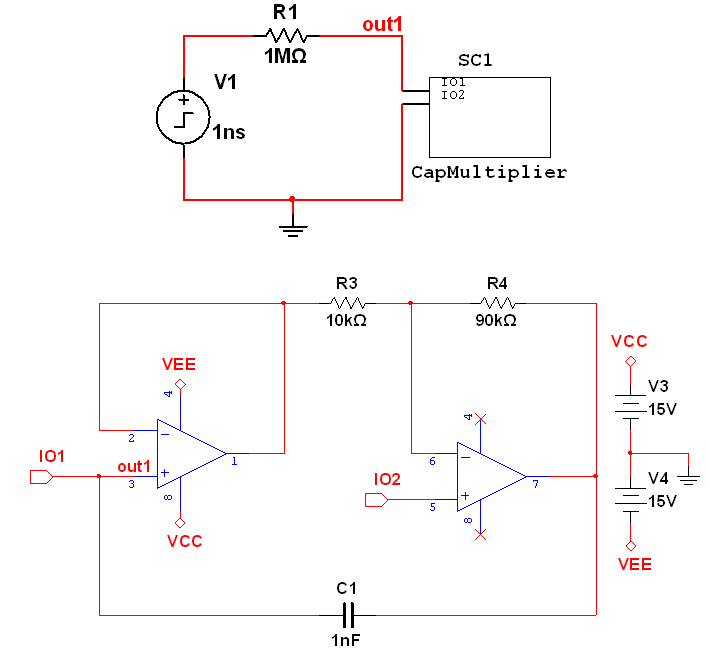
\includegraphics[scale=0.8]{figure4}
			\caption{}
			\label{fig:pic4}
		\end{figure}
	
		De la ecuación (\ref{E:eq2}) tenemos que
		\begin{align}
			V_o(s) = -\frac{R_2}{R_1}V_i(s) = -\frac{90k\Omega}{10k\Omega}(1) = -9V\nonumber
		\end{align}
		
		Por lo que el amplificador operacional no alcanza a saturarse.
		La constante de tiempo será ahora de
		\begin{align}
			\tau = RC_{eq} = (1\times 10^{6})(10\times 10^{-9}) = 10 ms\nonumber
		\end{align}
	
		Así, la nueva ecuación para el voltaje en el capacitor es
		\begin{align}
			v_c(t) = 1 - e^{-100t}
		\end{align}
	
		Por lo que ahora al capacitor le tomará aproximadamente $(6\tau=60ms)$ para cargarse
		En la figura \ref{fig:pic5} se muestra la gráfica del nuevo voltaje de carga en el capacitor
		\begin{figure}[H]
			\centering
			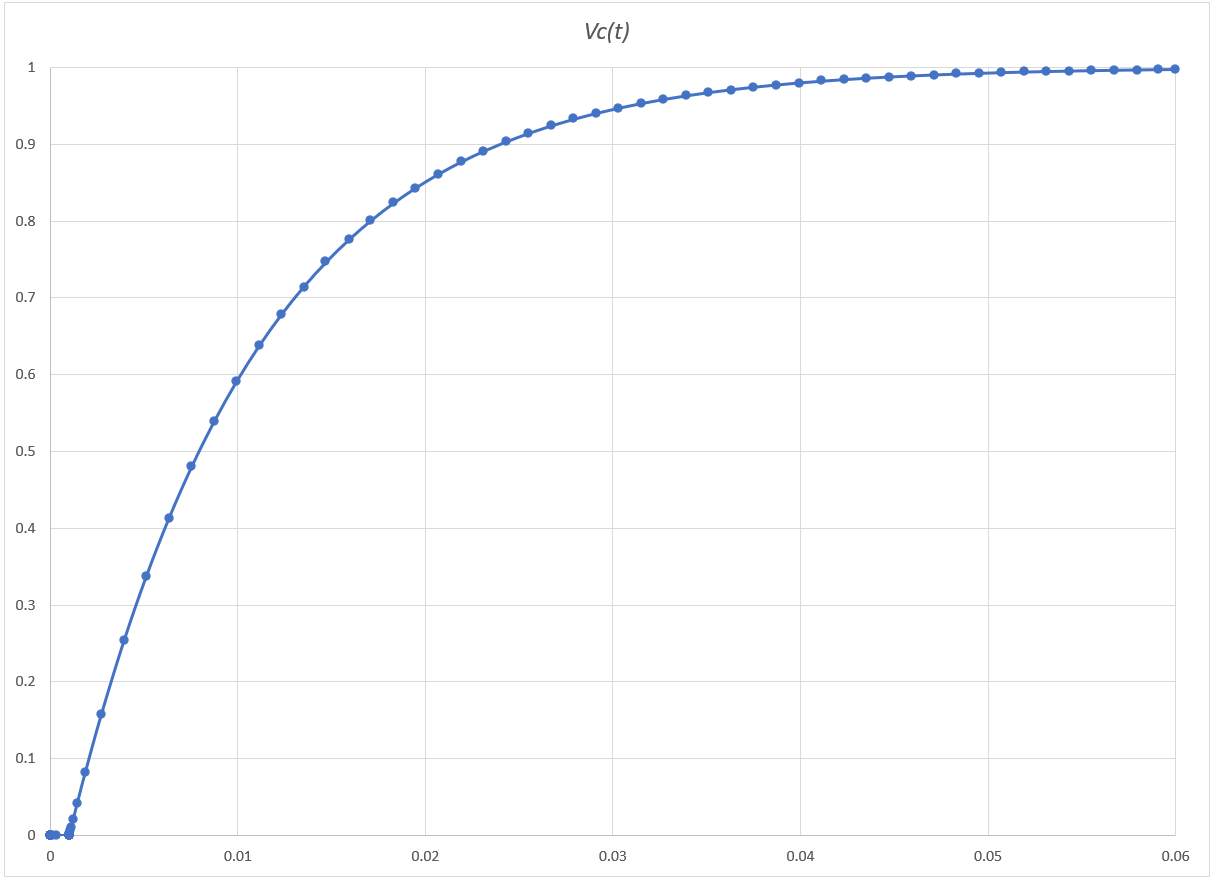
\includegraphics[scale=0.5]{figure5}
			\caption{Voltaje de carga para $C_{eq} = 10nF$}
			\label{fig:pic5}
		\end{figure}
		\begin{figure}[H]
			\centering
			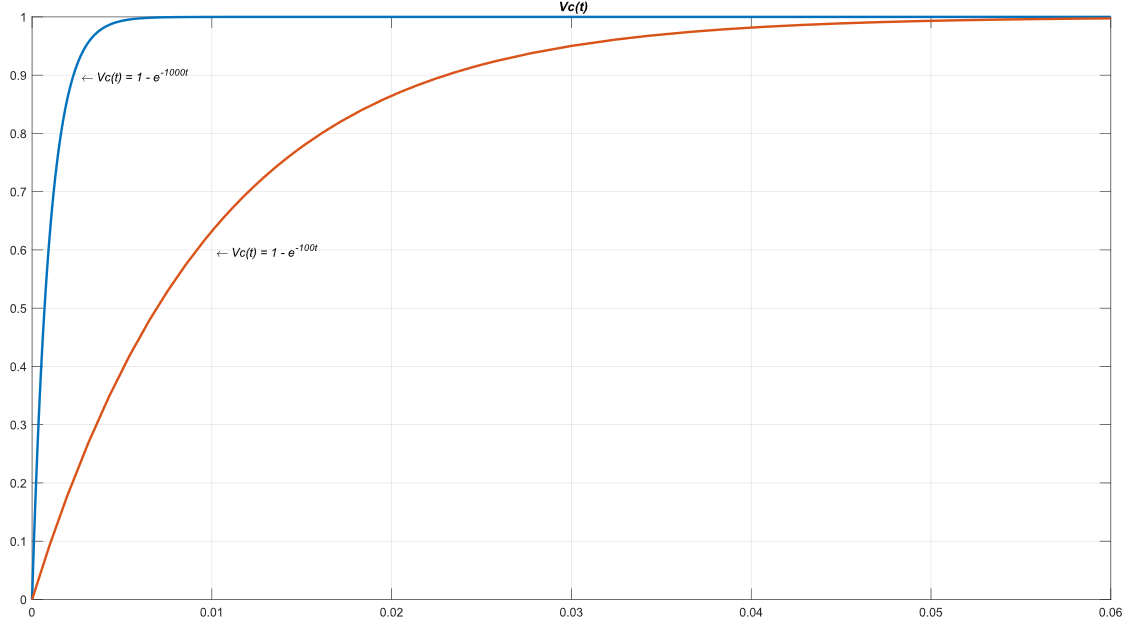
\includegraphics[scale=0.66]{figure6}
			\caption{Diferencia entre los distintos voltajes de carga}
			\label{fig:pic6}
		\end{figure}
	\end{myexample}
\end{document}